\documentclass{article}
\usepackage{graphicx} % Required for inserting images
\usepackage{amsmath}
\usepackage{amssymb}
\usepackage{epstopdf}
\usepackage{inputenc}
\usepackage{geometry}
\usepackage{biblatex}
\usepackage{algorithm}
\usepackage{algpseudocode}
\usepackage{float} 
\usepackage{hyperref}
\usepackage{booktabs}
\usepackage{subfig}
\usepackage{enumitem}
\usepackage{listings}
\usepackage{xcolor}
\usepackage{multirow}

\geometry{left=2.5cm,right=2.5cm,top=2.5cm,bottom=2.5cm}
\addbibresource{bibliography.bib}
\graphicspath{{figures/}}

% Configuration of code blocks with the listings package
\lstset{
  basicstyle=\ttfamily\small,
  keywordstyle=\color{blue},
  commentstyle=\color{green!50!black},
  stringstyle=\color{red},
  showstringspaces=false,
  breaklines=true,
  frame=single, 
  numbers=left, 
  numberstyle=\tiny\color{gray}, 
  stepnumber=1, 
  numbersep=5pt, 
  tabsize=2, 
  captionpos=b, 
}

\title{\textbf{Process Mining: Recommendation System} \\ {\Large Predictive Process Monitoring with Decision Trees}}
\author{Giorgia Gabardi (257838)}
\date{}
\begin{document}

\maketitle % Print the title section


\begin{abstract}
\noindent
This project implements a recommendation system for predictive process monitoring based on decision tree classifiers. The system analyzes a real-world production event log to predict whether an ongoing process instance will lead to a positive outcome (fast: cycle time below average) or a negative outcome (slow: cycle time above average). For traces predicted as negative, recommendations are extracted from the decision tree, suggesting which activities should be performed---or avoided---to improve the expected outcome. The approach uses boolean encoding of prefix traces and includes a padding mechanism for shorter traces. Performance is evaluated both in terms of predictive accuracy (using standard classification metrics) and recommendation quality (using a dedicated evaluation metric that checks whether the recommended activities are actually followed in the complete traces). Results are compared across different prefix lengths to assess how early information availability affects both prediction and recommendation effectiveness.
\end{abstract}

\hspace*{3.6mm}\textit{Keywords:} process mining, predictive monitoring, decision trees, recommendations, machine learning.


\section{Introduction}

In many real-world processes, it is useful to predict as early as possible whether an ongoing case will end positively or negatively, and to suggest corrective actions when a negative outcome is expected.

\medskip
\noindent
This work focuses on applying decision tree models to a real-world production log from a manufacturing setting with the goal of supporting predictive process monitoring. In particular, the study aims to:
\begin{itemize}
    \item \textbf{Outcome Prediction}: Train a decision tree classifier to predict whether an ongoing process instance (represented as a trace prefix) will result in a positive or negative outcome.
    \item \textbf{Recommendation Generation}: For traces predicted to have negative outcomes, extract recommendations indicating which activities should be performed to achieve a positive result.
    \item \textbf{Evaluation}: Assess both the predictive accuracy of the classifier and the effectiveness of the generated recommendations.
\end{itemize}

\noindent
The production log is labeled based on cycle time: traces with cycle time below the average are labeled as positive (\textit{true}), while those above average are labeled as negative (\textit{false}). The challenge is to predict this outcome using only partial trace information (prefixes) and to recommend corrective actions when necessary. Special attention is given to the handling of traces shorter than the chosen prefix length through proper padding, and to the exclusion of technical artifacts (such as trace identifiers and prefix length) from the feature space to ensure meaningful predictions. Finally, the prediction and recommendation results are compared across different prefix lengths to evaluate the trade-off between early intervention and information availability.


\section{Implementation}

The recommendation system was implemented in Python, using the \textit{PM4Py} library for process mining operations and \textit{scikit-learn} for machine learning. The code is organized into four modules:
\begin{itemize}
    \item \texttt{preprocessing.py}: log import, prefix generation with padding, activity extraction, and boolean encoding.
    \item \texttt{types.py}: data structures for tree conditions (\texttt{BooleanCondition}, \texttt{ThresholdCondition}).
    \item \texttt{tree\_utils.py}: DFS traversal, path confidence computation, compliance filtering, and missing condition extraction.
    \item \texttt{recommendations.py}: the main \texttt{extract\_recommendations} and \texttt{evaluate\_recommendations} functions.
\end{itemize}

\noindent
The pipeline is executed in a Jupyter Notebook (\texttt{tutorial\_completo.ipynb}) that sequentially calls each stage, from data loading to the final comparison across prefix lengths.

\subsection{Data Loading and Preprocessing}

\subsubsection{Event Log Import}

The event logs, provided in XES format, are imported using PM4Py and converted into \texttt{EventLog} objects for further processing. The dataset is pre-split into training (80\%) and testing (20\%) sets:
\begin{itemize}
    \item \texttt{Production\_avg\_dur\_training\_0-80.xes}: Training set containing 177 traces
    \item \texttt{Production\_avg\_dur\_testing\_80-100.xes}: Test set containing 43 traces
\end{itemize}

\subsubsection{Prefix Extraction with Padding}

Since the goal is to make predictions on ongoing (incomplete) traces, each complete trace is truncated to a fixed \textit{prefix\_length} representing the number of events observed so far. This is important because it simulates the real-world scenario where decisions must be made before the process completes.

\paragraph{Padding Strategy:}
When working with trace prefixes, some process instances may contain fewer events than the selected prefix length. A padding mechanism is applied so that each trace is encoded with the same number of features.
This choice prevents:
\begin{enumerate}
\item The exclusion of shorter traces from the analysis
\item A potential bias toward longer process instances
\item Inconsistencies in the structure of the feature matrix
\end{enumerate}

\noindent
The padding is implemented by adding special \texttt{PADDING} events to traces shorter than the required prefix length. The padding procedure is summarized in the following pseudocode:
\begin{algorithm}[H]
\caption{Prefix Creation with Padding}
\label{alg:prefix-padding}
\begin{algorithmic}[1]
\Require $log$ \Comment{Original event log}
\Require $prefix\_length$ \Comment{Target prefix length}
\Require $use\_padding$ \Comment{Boolean flag for padding shorter traces}
\Ensure $prefixes\_log$ \Comment{Event log with prefixes of uniform length}

\State $prefixes\_log \gets$ empty log
\For{each $trace$ in $log$}
    \State $prefix\_trace \gets$ first $prefix\_length$ events of $trace$
    \If{$use\_padding$ AND length($prefix\_trace$) $<$ $prefix\_length$}
        \While{length($prefix\_trace$) $<$ $prefix\_length$}
            \State Append a special event \texttt{PADDING} to $prefix\_trace$
        \EndWhile
    \EndIf
    \State Append $prefix\_trace$ to $prefixes\_log$
\EndFor
\State \Return $prefixes\_log$
\end{algorithmic}
\end{algorithm}

\subsection{Activity Extraction and Boolean Encoding}

\subsubsection{Feature Space Definition}

To construct the feature space, all unique activity names are extracted from the complete training log (rather than the prefixed version). This ensures that every possible activity in the process is represented as a feature, even if some activities do not appear in every trace. The extraction is performed by scanning each trace in the log and collecting activity names in the order they appear, while avoiding duplicates. 

\subsubsection{Boolean Encoding}

Once the prefixed traces are created, they are transformed into a tabular format suitable for machine learning. In this representation, each row corresponds to a trace, and each column represents a specific activity from the feature space. A boolean value indicates whether the activity is present (True) or absent (False) in the trace prefix. Additional columns store the trace identifier, the prefix length and the ground truth label indicating the outcome of the trace.

\subsubsection{Validation} After the boolean encoding, several checks are performed to ensure data integrity:
\begin{itemize}
    \item All traces have a prefix length equal to the specified value.
    \item The total number of encoded traces matches the number of input traces.
    \item The special \texttt{PADDING} activity is correctly included for traces that required padding.
\end{itemize}

\noindent
This encoding allows the decision tree model to process the traces as structured feature vectors, preserving information about the activities present in each prefix.

\subsection{Feature Engineering and Training Preparation}

\subsubsection{Feature Selection}

An important choice is which columns to use as features for the decision tree. The encoded DataFrame contains:
\begin{itemize}
    \item \texttt{trace\_id}: Technical identifier (must be excluded)
    \item \texttt{prefix\_length}: Length of the prefix (must be excluded)
    \item Activity columns: Boolean indicators (features for training)
    \item \texttt{label}: Ground truth (target variable)
\end{itemize}

\noindent
\textbf{Note}: The \texttt{prefix\_length} column is included in the encoded DataFrame for validation purposes, but it should not be used as a feature. It represents a technical artifact rather than a characteristic of the process, is constant across traces when padding is applied, has no meaningful connection to the outcome and could prevent the model from generalizing to different prefix lengths.



\subsection{Decision Tree Training and Hyperparameter Optimization}

The feature matrix $X$ is constructed by selecting only the boolean activity columns from the encoded DataFrame, while the columns \texttt{trace\_id}, \texttt{prefix\_length} and \texttt{label} are excluded. The label column is used as the target variable $y$. The same procedure is applied to both the training and test sets, and consistency checks are performed to ensure dimensional alignment and that no technical artifact is included among the features.

\subsubsection{Hyperparameter Optimization}

Before training the final model, a grid search with 5-fold cross-validation (\texttt{GridSearchCV}) is optionally performed to identify the best combination of hyperparameters. The search space includes:

\begin{itemize}
    \item \texttt{max\_depth}: controls the maximum depth of the tree, limiting its complexity.
    \item \texttt{criterion}: the splitting criterion (\textit{gini} impurity or \textit{entropy}).
    \item \texttt{max\_features}: the number of features considered at each split (\textit{None}, \textit{sqrt}, \textit{log2}).
    \item \texttt{min\_samples\_split} and \texttt{min\_samples\_leaf}: minimum number of samples required to split an internal node and to form a leaf, respectively.
\end{itemize}

\noindent
All combinations are evaluated exhaustively, and the configuration achieving the highest F1-score across the cross-validation folds is selected. A fixed random seed is used throughout to ensure reproducibility.

\subsubsection{Model Training}

If hyperparameter optimization is applied, the best parameters found by the grid search are used; otherwise, a set of default parameters is used (e.g., limited tree depth, Gini criterion). The decision tree is then trained on the full training set using scikit-learn's \texttt{DecisionTreeClassifier}. After training, the resulting tree depth and number of leaves are reported to assess the model's complexity.

\subsection{Decision Tree Visualization}

After training, the decision tree is exported and visualized using the \texttt{graphviz} library. This visualization helps understand the internal logic of the model: it shows the feature used at each decision node, the split threshold, the class distribution at each node and the predicted class at each leaf.

\medskip
\noindent
Since the features are boolean (activity presence), each internal node represents a question of the form \textit{``Is activity X present in the trace prefix?''} The left branch corresponds to \textit{False} (activity absent) and the right branch corresponds to \textit{True} (activity present). The leaves display the predicted class (\textit{true} for fast traces, \textit{false} for slow traces) along with the proportion of training samples reaching that node. The tree is rendered with colored nodes: blue shades indicate majority negative class, orange shades indicate majority positive class, with intensity proportional to class purity.


\subsection{Prediction and Model Evaluation}

\subsubsection{Test Set Predictions}

The trained decision tree classifier is used to generate predictions on the test set. Each test trace prefix, encoded using the same boolean encoding scheme as the training set, is classified as either \textit{true} (fast) or \textit{false} (slow):
\[
\hat{y}_i = \text{clf.predict}(\mathbf{x}_i), \quad \forall \, i \in \{1, \dots, n_{\text{test}}\}
\]

\subsubsection{Performance Metrics}

Standard classification metrics are computed to evaluate the predictive accuracy of the model. For a binary classification task with positive label \textit{true} and negative label \textit{false}, the following metrics are used:

\begin{itemize}
    \item \textbf{Accuracy}: fraction of correctly classified instances.
    \[
    \text{Accuracy} = \frac{TP + TN}{TP + TN + FP + FN}
    \]
    \item \textbf{Precision}: fraction of predicted positives that are truly positive.
    \[
    \text{Precision} = \frac{TP}{TP + FP}
    \]
    \item \textbf{Recall}: fraction of actual positives that are correctly identified.
    \[
    \text{Recall} = \frac{TP}{TP + FN}
    \]
    \item \textbf{F1-Score}: harmonic mean of precision and recall.
    \[
    F_1 = 2 \cdot \frac{\text{Precision} \cdot \text{Recall}}{\text{Precision} + \text{Recall}}
    \]
\end{itemize}

\subsubsection{Confusion Matrix}

The confusion matrix is computed with explicit label ordering (\texttt{labels=['false', 'true']}) to ensure correct interpretation of the results:

\begin{center}
\begin{tabular}{cc|c|c|}
& \multicolumn{1}{c}{} & \multicolumn{2}{c}{\textbf{Predicted}} \\
& \multicolumn{1}{c}{} & \multicolumn{1}{c}{Negative}  & \multicolumn{1}{c}{Positive} \\\cline{3-4}
\multirow{2}{*}{\textbf{Actual}} & Negative (\textit{false}) & TN & FP \\\cline{3-4}
                        & Positive (\textit{true})  & FN & TP \\\cline{3-4}
\end{tabular}
\end{center}

\noindent
Where:
\begin{itemize}
    \item \textbf{TN (True Negatives)}: Slow traces correctly predicted as slow.
    \item \textbf{FP (False Positives)}: Slow traces incorrectly predicted as fast.
    \item \textbf{FN (False Negatives)}: Fast traces incorrectly predicted as slow.
    \item \textbf{TP (True Positives)}: Fast traces correctly predicted as fast.
\end{itemize}



\subsection{Recommendation Generation}

The main part of this project is the generation of recommendations for traces predicted as negative. The goal is to suggest which activities should be performed (or avoided) to push the process towards a positive outcome. The recommendation algorithm uses the internal structure of the trained decision tree.

\subsubsection{Data Structures}

Two types of conditions are used to represent the decision rules extracted from the tree:

\begin{itemize}
    \item \textbf{BooleanCondition}: Represents a condition on a boolean feature (activity), defined by the activity name and the required value (\textit{True} = activity should be present, \textit{False} = activity should be absent).
    \item \textbf{ThresholdCondition}: Represents a numerical condition (used internally for \texttt{prefix\_length} if it were included as feature), defined by the feature name, a comparison operator ($\leq$ or $>$) and a threshold value.
\end{itemize}

\noindent
A \textit{path} is defined as a sequence of conditions from the root of the tree to a leaf node. Each path encodes a set of requirements that, if satisfied, lead to the class predicted by the corresponding leaf.

\subsubsection{Algorithm Overview}

The recommendation extraction process follows four main steps:

\begin{enumerate}
    \item \textbf{Extract Positive Paths}: Traverse the decision tree using Depth-First Search (DFS) to identify all root-to-leaf paths that lead to a positive prediction.
    \item \textbf{Filter Compliant Paths}: For each negatively predicted trace, select only the positive paths whose conditions do not contradict the current state of the trace.
    \item \textbf{Select Best Path}: Among the compliant paths, choose the one with the highest confidence (and shortest length in case of ties).
    \item \textbf{Extract Missing Conditions}: Compare the selected path's conditions with the trace's current state to identify the activities that need to change.
\end{enumerate}

\subsubsection{Step 1: Extracting Positive Paths via DFS}

The decision tree is traversed using a recursive Depth-First Search starting from the root node. At each internal node, the algorithm records the splitting condition (which activity is tested and in which direction) and recurses into both children. When a leaf node is reached, the algorithm checks whether the predicted class is positive. If so, the accumulated path of conditions is saved together with a confidence score.

\medskip
\noindent
The \textbf{confidence} of a leaf node $\ell$ is defined as the class probability of the positive class at that leaf:
\[
\text{confidence}(\ell) = \frac{n_{\text{positive}}(\ell)}{n_{\text{samples}}(\ell)}
\]
where $n_{\text{positive}}(\ell)$ is the number of positive-class samples in the leaf and $n_{\text{samples}}(\ell)$ is the total number of training samples reaching that leaf. In other words, it is the fraction of training instances at the leaf that belong to the positive class.

\medskip
\noindent
Note that since \texttt{prefix\_length} is excluded from the features, the DFS encounters only boolean splits. However, the implementation also supports threshold-based splits (via \texttt{ThresholdCondition}) for generality.

\begin{algorithm}[H]
\caption{Extract Positive Paths (DFS)}
\label{alg:positive-paths}
\begin{algorithmic}[1]
\Require $tree$ \Comment{Trained Decision Tree}
\Require $feature\_names$ \Comment{List of feature names}
\Require $positive\_class\_idx$ \Comment{Index of positive class in tree.classes\_}
\Ensure $paths$ \Comment{List of (path, confidence) for positive leaves}

\State $paths \gets$ empty list
\Function{DFS}{$node$, $current\_path$}
    \If{$node$ is a leaf}
        \If{$\arg\max$ of class counts at $node$ $=$ $positive\_class\_idx$}
            \State $conf \gets n_{\text{positive}}(node) \;/\; n_{\text{samples}}(node)$
            \State Append ($current\_path$, $conf$) to $paths$
        \EndIf
        \State \Return
    \EndIf
    \State $feat \gets$ feature at $node$
    \State \Call{DFS}{left child, $current\_path$ + [BooleanCondition($feat$, False)]}
    \State \Call{DFS}{right child, $current\_path$ + [BooleanCondition($feat$, True)]}
\EndFunction
\State \Call{DFS}{root, empty list}
\State \Return $paths$
\end{algorithmic}
\end{algorithm}

\subsubsection{Step 2: Filtering Compliant Paths}

Given a trace predicted as negative, not all positive paths are reachable: some may require conditions that contradict the current state of the trace. A path is said to be \textit{compliant} with a trace if none of its conditions contradict the trace's current feature values.

\medskip
\noindent
A condition \textit{contradicts} a trace if the condition requires an activity to have a specific value (present or absent), but the trace already has the opposite value. Crucially, if a condition requires an activity that is \textit{not yet present} in the trace, this is not considered a contradiction---it represents a potential future action that could still happen.

\medskip
\noindent
Formally, let $P = \{c_1, c_2, \dots, c_k\}$ be a positive path and $\mathbf{t}$ the current trace state. The path is compliant if:
\[
\forall \, c_i \in P: \; \neg \, \text{contradicts}(c_i, \mathbf{t})
\]

\subsubsection{Step 3: Selecting the Best Path}

Among all compliant paths, the algorithm selects the one that offers the highest confidence. In case of ties, the path with fewer conditions (i.e., shorter length) is preferred, as it requires fewer changes to the trace:
\[
P^* = \arg\max_{P \in \mathcal{C}} \left( \text{confidence}(P), \; -|P| \right)
\]
where $\mathcal{C}$ is the set of compliant paths and $|P|$ is the number of conditions in the path.

\subsubsection{Step 4: Extracting Missing Conditions (Recommendations)}

Once the best compliant path is selected, the algorithm compares each of its boolean conditions against the trace's current state. For each condition, the actual value of the activity in the trace is determined: if the activity is present in the trace's feature dictionary it is \textit{True}; if it is absent (not in the dictionary), it defaults to \textit{False}. A condition is \textit{missing} if the required value differs from the actual value:

\[
\text{Recommendations}(\mathbf{t}, P^*) = \left\{ c \in P^* \;\middle|\; c.\text{value} \neq \mathbf{t}.\text{get}(c.\text{feature},\; \text{False}) \right\}
\]

\noindent
Each recommendation is a \texttt{BooleanCondition} indicating:
\begin{itemize}
    \item If \texttt{value = True}: the activity should be \textbf{added} (i.e., performed in the future steps of the process).
    \item If \texttt{value = False}: the activity should be \textbf{avoided} (i.e., it is detrimental to a positive outcome).
\end{itemize}

\subsubsection{Complete Recommendation Pipeline}

The full recommendation pipeline is implemented in the function \texttt{extract\_recommendations(tree, feature\_names, class\_values, prefix\_set)}, summarized in Algorithm~\ref{alg:recommendations}.

\begin{algorithm}[H]
\caption{Extract Recommendations}
\label{alg:recommendations}
\begin{algorithmic}[1]
\Require $tree$ \Comment{Trained Decision Tree}
\Require $feature\_names$ \Comment{Feature names}
\Require $class\_values$ \Comment{[\textit{positive\_class}, \textit{negative\_class}]}
\Require $prefix\_set$ \Comment{Boolean-encoded test set}
\Ensure $recommendations$ \Comment{Dictionary mapping traces to recommendations}

\State $positive\_class \gets class\_values[0]$
\State $positive\_class\_idx \gets$ index of $positive\_class$ in $tree.classes\_$
\State $positive\_paths \gets$ \Call{ExtractPositivePaths}{$tree$, $feature\_names$, $positive\_class\_idx$}
\State $predictions \gets tree.\text{predict}(prefix\_set[feature\_names])$
\State $recommendations \gets$ empty dictionary

\For{each prefix trace $\mathbf{t}_i$ in $prefix\_set$}
    \State $key_i \gets$ frozenset of activities present in $\mathbf{t}_i$
    \If{$predictions[i] = positive\_class$}
        \State $recommendations[key_i] \gets \emptyset$ \Comment{Already positive, empty set}
        \State \textbf{continue}
    \EndIf
    \State $current\_state \gets$ activities with value True in $\mathbf{t}_i$
    \State $compliant \gets$ \Call{FilterCompliantPaths}{$positive\_paths$, $current\_state$}
    \If{$compliant$ is empty}
        \State $recommendations[key_i] \gets \emptyset$ \Comment{No viable path, empty set}
        \State \textbf{continue}
    \EndIf
    \State $P^* \gets \arg\max_{P \in compliant} \left( \text{confidence}(P), -|P| \right)$
    \State $missing \gets$ \Call{GetMissingConditions}{$P^*$, $current\_state$}
    \State $recommendations[key_i] \gets missing$
\EndFor
\State \Return $recommendations$
\end{algorithmic}
\end{algorithm}

\noindent
The function predicts the label internally using the tree, so the input \texttt{prefix\_set} only needs to be the boolean-encoded DataFrame (including \texttt{trace\_id}, \texttt{label}, \texttt{prefix\_length} columns, which are ignored during prediction). The output is a dictionary where each key is a frozenset of the activities currently present in the trace prefix, and the associated value is:
\begin{itemize}
    \item An \textbf{empty set}: if the trace was predicted as positive (no recommendation needed), or if no compliant positive path was found (no viable recommendation).
    \item A \textbf{set of BooleanCondition} objects: the recommended changes to reach a positive outcome.
\end{itemize}

%------------------------------------------------

\subsection{Recommendation Evaluation}

To assess the quality of the generated recommendations, the function \texttt{evaluate\_recommendations} compares the recommended activities against the \textit{complete} (non-truncated) test traces. The intuition is: if the system recommends that an activity should be present, we check whether that activity \textit{actually occurs} in the full trace and whether the trace's ground-truth outcome is positive.

\subsubsection{Evaluation Criteria}

The evaluation is performed only on traces with a \textbf{negative prediction} (since positive predictions receive no recommendation). For each such trace, the algorithm:
\begin{enumerate}
    \item Looks up the recommendation in the dictionary (using the prefix's activity frozenset as key).
    \item Boolean-encodes the \textit{complete} test trace (not just the prefix).
    \item Checks whether \textbf{all recommended conditions are satisfied} in the complete trace:
    \begin{itemize}
        \item For each condition with \texttt{value = True}: the activity must be present in the full trace.
        \item For each condition with \texttt{value = False}: the activity must be absent from the full trace.
    \end{itemize}
    \item If all conditions are met, the recommendation is considered \textit{followed}; otherwise, it is \textit{not followed}.
    \item If the recommendation set is empty (no recommendation could be generated), it is classified as \textit{not followed}.
\end{enumerate}

\noindent
Based on this, each evaluated trace is classified into one of four categories:

\begin{center}
\begin{tabular}{cc|c|c|}
& \multicolumn{1}{c}{} & \multicolumn{2}{c}{\textbf{Ground Truth Outcome}} \\
& \multicolumn{1}{c}{} & \multicolumn{1}{c}{Negative (\textit{false})}  & \multicolumn{1}{c}{Positive (\textit{true})} \\\cline{3-4}
\multirow{2}{*}{\textbf{Recommendation}} & Followed     & FP & TP \\\cline{3-4}
                                          & Not Followed & TN & FN \\\cline{3-4}
\end{tabular}
\end{center}

\begin{itemize}
    \item \textbf{TP}: The recommendation was followed in the complete trace, and the ground-truth outcome is positive. This confirms the recommendation was correct.
    \item \textbf{TN}: The recommendation was not followed, and the ground-truth outcome is negative. The trace remained negative, consistent with not following the advice.
    \item \textbf{FP}: The recommendation was followed, but the ground-truth outcome is negative. The recommendation was misleading.
    \item \textbf{FN}: The recommendation was not followed, but the ground-truth outcome is positive. The trace achieved a positive outcome without the suggested intervention.
\end{itemize}

\subsubsection{Recommendation Metrics}

From this classification, the standard metrics are computed to obtain what we call the \textit{recommendation F-measure} ($F_{\text{rec}}$):

\[
\text{Precision}_{\text{rec}} = \frac{TP}{TP + FP}, \quad
\text{Recall}_{\text{rec}} = \frac{TP}{TP + FN}, \quad
F_{\text{rec}} = 2 \cdot \frac{\text{Precision}_{\text{rec}} \cdot \text{Recall}_{\text{rec}}}{\text{Precision}_{\text{rec}} + \text{Recall}_{\text{rec}}}
\]

\noindent
Additionally, the recommendation accuracy is computed as:
\[
\text{Accuracy}_{\text{rec}} = \frac{TP + TN}{TP + TN + FP + FN}
\]

\noindent
These metrics measure how well the recommendation system performs: high $F_{\text{rec}}$ indicates that the recommended activities were actually followed and led to positive outcomes.


\subsection{Qualitative Inspection of Recommendations}

Beyond quantitative evaluation, the notebook provides a qualitative analysis of the generated recommendations.

\subsubsection{Textual Analysis}

For each negatively predicted trace that received a recommendation, the system prints:
\begin{itemize}
    \item The set of activities currently present in the prefix.
    \item The recommended actions: activities to \textbf{add} (perform in the future) or to \textbf{remove} (avoid).
\end{itemize}

\noindent
A detailed example is presented for a specific trace, showing the mapping between the trace's current state and the suggested modifications.

\subsubsection{Visual Example on the Decision Tree}

To illustrate how recommendations relate to the tree's structure, a selected negative trace is visualized directly on the decision tree. The visualization highlights:
\begin{itemize}
    \item The \textbf{path of the trace} through the tree (orange border), showing which nodes are traversed given the trace's current feature values.
    \item The \textbf{recommendation nodes} (blue border for ADD, red border for REMOVE), indicating the tree nodes where the recommended features are tested.
    \item The \textbf{leaf node} where the trace ends up (negative prediction).
\end{itemize}

\noindent
This visualization shows clearly \textit{why} the trace received a negative prediction and \textit{what} the tree suggests to fix it. It also serves as a check to verify that the recommendation algorithm correctly identifies the relevant decision boundaries.

%------------------------------------------------

\subsection{Prefix Length Comparison}

To evaluate how the amount of available information affects both prediction and recommendation quality, the entire pipeline described above---from prefix generation through recommendation evaluation---is executed independently for every prefix length from 1 to 12. For each prefix length, a new decision tree is optimized via GridSearchCV and trained from scratch; predictions, recommendations, and evaluation metrics are collected into a summary dictionary.

%----------------------------------------------------------------------------------------
%	RESULTS
%----------------------------------------------------------------------------------------

\section{Results}

This section presents the experimental results obtained by applying the recommendation pipeline to the production event log. All results are reported for the default prefix length of 11, unless otherwise stated.

\subsection{Dataset Characteristics}

The production event log contains 220 traces in total, pre-split into a training set of 177 traces and a test set of 43 traces. Each trace represents a production process instance, labeled as \textit{true} (fast: cycle time below average) or \textit{false} (slow: cycle time above average).

\begin{center}
\begin{tabular}{lrrr}
\toprule
& \textbf{Training} & \textbf{Test} & \textbf{Total} \\
\midrule
Positive (\textit{true})  & 116 (65.5\%) & 32 (74.4\%) & 148 (67.3\%) \\
Negative (\textit{false}) &  61 (34.5\%) & 11 (25.6\%) &  72 (32.7\%) \\
\midrule
\textbf{Total}            & 177          & 43          & 220          \\
\bottomrule
\end{tabular}
\end{center}

\noindent
The dataset is imbalanced in favor of the positive class ($\sim$65--75\%), which is an important consideration for both model training and evaluation. After prefix extraction with padding at length 11, the boolean encoding produces 26 activity features per trace (plus \texttt{trace\_id}, \texttt{prefix\_length}, and \texttt{label}, which are excluded from training). The 26 distinct activities include machine-specific operations (e.g., \textit{Turning \& Milling -- Machine 8}), quality control steps (e.g., \textit{Turning \& Milling Q.C.}, \textit{Final Inspection Q.C.}), and an \textit{other} category.

\subsection{Hyperparameter Optimization}

GridSearchCV explored 216 parameter combinations over a 5-fold cross-validation with F1-score (\texttt{pos\_label='true'}) as the optimization criterion. The search space was:

\begin{center}
\begin{tabular}{ll}
\toprule
\textbf{Hyperparameter}        & \textbf{Values} \\
\midrule
\texttt{criterion}             & \texttt{gini}, \texttt{entropy} \\
\texttt{max\_depth}            & 2, 3, 4, 5 \\
\texttt{max\_features}         & \texttt{None}, \texttt{sqrt}, \texttt{log2} \\
\texttt{min\_samples\_split}   & 2, 5, 10 \\
\texttt{min\_samples\_leaf}    & 1, 2, 4 \\
\bottomrule
\end{tabular}
\end{center}

\noindent
The best parameters found for prefix length 11 are:

\begin{center}
\begin{tabular}{ll}
\toprule
\textbf{Parameter}             & \textbf{Best Value} \\
\midrule
\texttt{criterion}             & \texttt{entropy} \\
\texttt{max\_depth}            & 2 \\
\texttt{max\_features}         & \texttt{None} \\
\texttt{min\_samples\_leaf}    & 1 \\
\texttt{min\_samples\_split}   & 2 \\
\bottomrule
\end{tabular}
\end{center}

\noindent
The best cross-validated F1-score on the training set was \textbf{0.822}. The selection of \texttt{max\_depth} = 2 indicates that the optimal model is a very shallow tree with only 4 leaves, which favors interpretability and avoids overfitting. The choice of \texttt{entropy} as the splitting criterion suggests that information gain provides better class separation for this dataset.

\subsection{Decision Tree Prediction Performance}

The trained decision tree (depth 2, 4 leaves) was evaluated on the 43 test traces with prefix length 11. The confusion matrix and derived metrics are reported below.

\subsubsection{Confusion Matrix}

\begin{center}
\begin{tabular}{cc|c|c|c}
& \multicolumn{1}{c}{} & \multicolumn{2}{c}{\textbf{Predicted}} & \\
& \multicolumn{1}{c}{} & \multicolumn{1}{c}{Negative}  & \multicolumn{1}{c}{Positive} & \multicolumn{1}{c}{\textbf{Total}} \\\cline{3-4}
\multirow{2}{*}{\textbf{Actual}} & Negative (\textit{false}) & 5 & 6 & 11 \\\cline{3-4}
                        & Positive (\textit{true})  & 2 & 30 & 32 \\\cline{3-4}
\multicolumn{2}{c|}{\textbf{Total}} & 7 & 36 & 43 \\
\end{tabular}
\end{center}

\subsubsection{Classification Metrics}

\begin{center}
\begin{tabular}{lr}
\toprule
\textbf{Metric} & \textbf{Value} \\
\midrule
Accuracy  & 0.814 \\
Precision & 0.833 \\
Recall    & 0.938 \\
F1-Score  & 0.882 \\
\bottomrule
\end{tabular}
\end{center}

\noindent
The model achieves an accuracy of 81.4\% and an F1-score of 0.882 on the test set. The model achieves a high recall of 0.938 which means that the model correctly identifies 93.8\% of the truly fast traces. The precision of 0.833 indicates that among the 36 traces predicted as positive, 30 are actually positive while 6 are false positives (slow traces incorrectly predicted as fast). Only 2 fast traces are missed (false negatives), confirming the model's strength in detecting positive outcomes. The relatively high number of false positives (6 out of 11 actual negatives) is likely due to the dataset imbalance and the limited depth of the tree. In practice, a false positive means a trace predicted as fast does not receive a recommendation. This is less problematic than a false negative, where a fast trace would receive an unnecessary recommendation.

\begin{figure}[H]
    \centering
    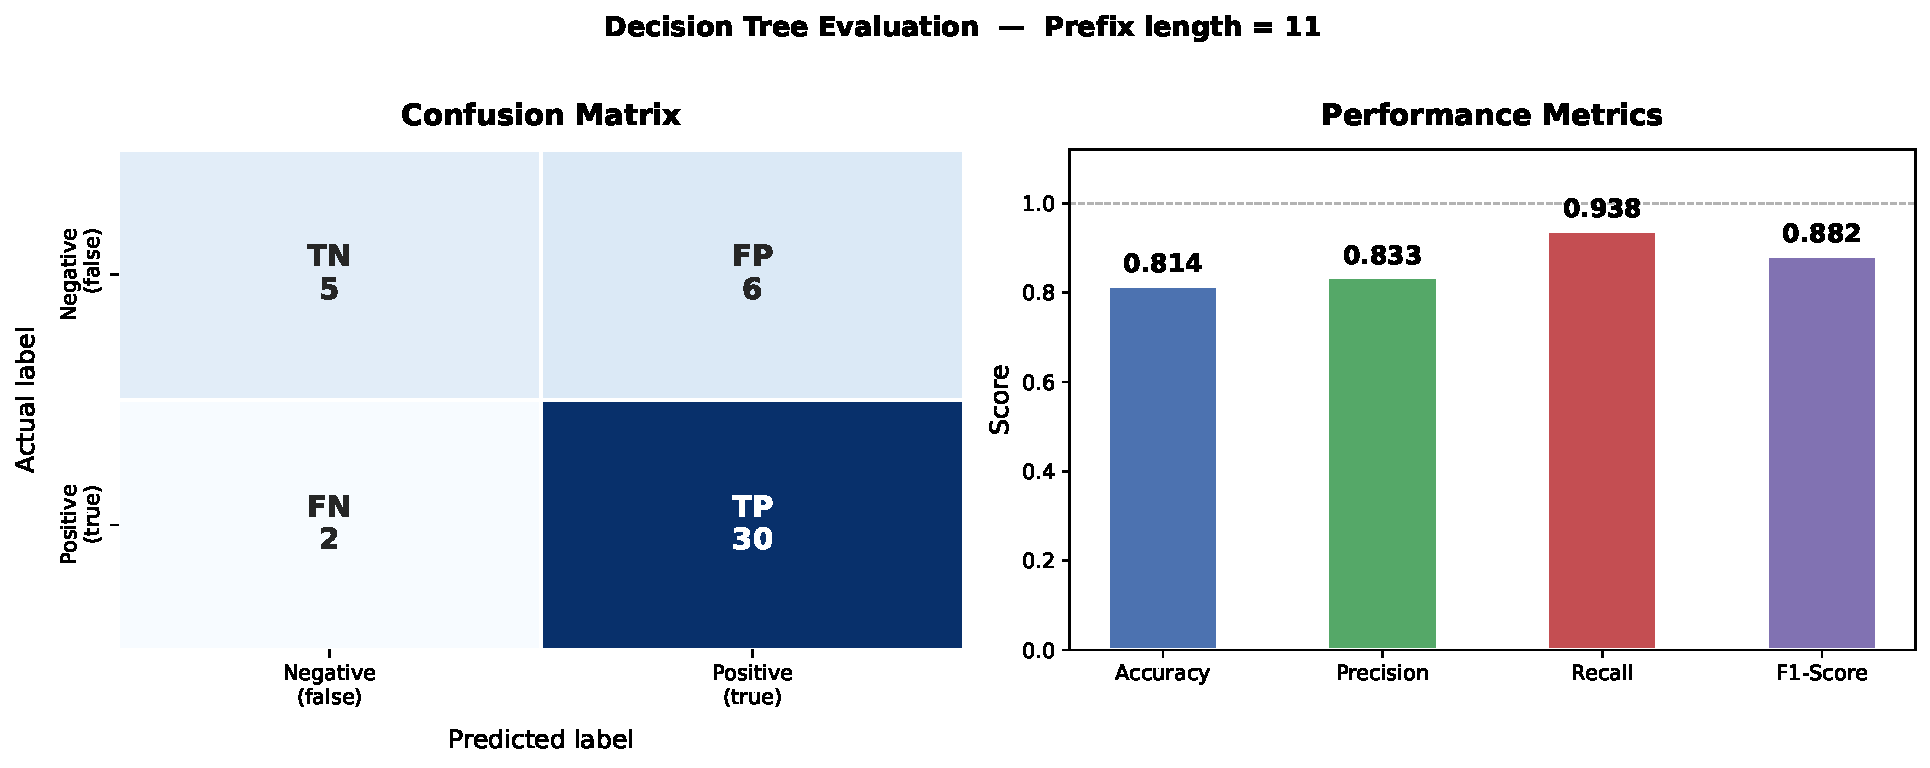
\includegraphics[width=\textwidth]{tree_evaluation.pdf}
    \caption{Decision tree evaluation on the test set (prefix length~=~11). \textbf{Left}: Confusion matrix showing the distribution of predictions. \textbf{Right}: Bar chart of the four classification metrics. The model achieves high recall (0.938) at the cost of moderate precision (0.833).}
    \label{fig:tree-evaluation}
\end{figure}

\subsection{Tree Structure and Key Splitting Features}

The optimized tree has depth 2 with 4 leaf nodes. The root node splits on \textbf{Laser Marking -- Machine 7}: traces that include this activity are routed to the right subtree, while those without it go to the left. At depth 2:

\begin{itemize}
    \item \textbf{Left subtree} (Laser Marking -- Machine 7 = False): splits on \textbf{Turning Q.C.}
    \begin{itemize}
        \item No Turning Q.C. $\Rightarrow$ Leaf: \textit{true} (positive)
        \item With Turning Q.C. $\Rightarrow$ Leaf: \textit{false} (negative)
    \end{itemize}
    \item \textbf{Right subtree} (Laser Marking -- Machine 7 = True): splits on \textbf{Final Inspection Q.C.}
    \begin{itemize}
        \item No Final Inspection Q.C. $\Rightarrow$ Leaf: \textit{false} (negative)
        \item With Final Inspection Q.C. $\Rightarrow$ Leaf: \textit{true} (positive)
    \end{itemize}
\end{itemize}

\noindent
This structure reveals that \textit{Laser Marking -- Machine 7} is the most discriminative feature at the process level. Among traces that pass through laser marking, the presence of \textit{Final Inspection Q.C.} is the key differentiator for a positive outcome. Among traces that do not involve laser marking, the absence of \textit{Turning Q.C.} is associated with faster completion.

\begin{figure}[H]
    \centering
    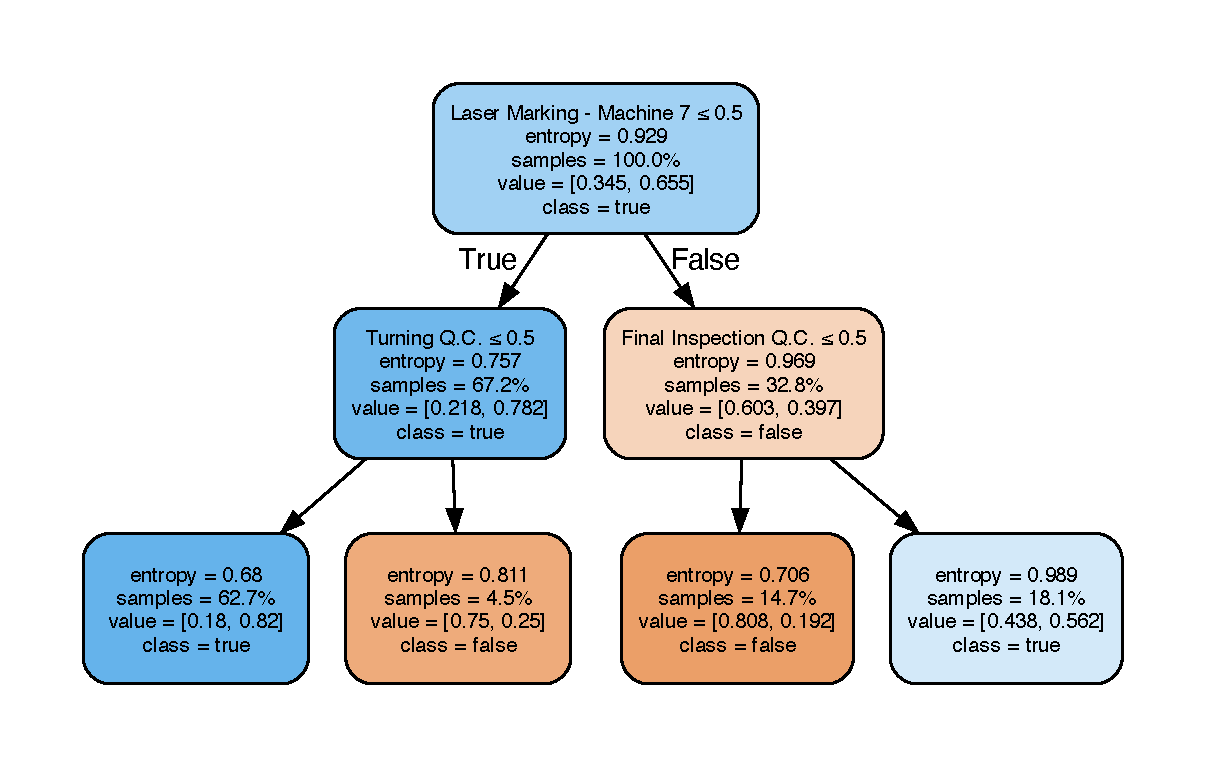
\includegraphics[width=0.85\textwidth]{decision_tree.pdf}
    \caption{Decision tree trained with optimized parameters (\texttt{criterion=entropy}, \texttt{max\_depth=2}).}
    \label{fig:decision-tree}
\end{figure}

\subsection{Recommendation Results}

\subsubsection{Summary Statistics}

Out of 43 test traces, the decision tree predicted 36 as positive and 7 as negative. The recommendation algorithm was applied to all 7 negatively predicted traces:

\begin{center}
\begin{tabular}{lr}
\toprule
\textbf{Category} & \textbf{Count} \\
\midrule
Positive predictions (no recommendation) & 36 \\
Negative predictions with recommendations & 7 \\
Negative predictions without viable path  & 0 \\
\midrule
\textbf{Total} & 43 \\
\bottomrule
\end{tabular}
\end{center}

\noindent
All 7 negatively predicted traces received at least one recommendation, meaning the algorithm always found a compliant positive path through the tree. The DFS traversal identified 2 positive paths in the tree (corresponding to the 2 positive leaves).

\subsubsection{Content of the Recommendations}

The recommendations generated for the 7 negative traces converge on a consistent pattern:

\begin{itemize}
    \item \textbf{4 traces} received a single recommendation: \textbf{Add \textit{Final Inspection Q.C.}} These are traces that already contain \textit{Laser Marking -- Machine 7} but lack the quality control step.
    \item \textbf{3 traces} received two recommendations: \textbf{Add \textit{Laser Marking -- Machine 7}} and \textbf{Add \textit{Final Inspection Q.C.}} These are traces that contain \textit{Turning Q.C.} but lack both key activities from the positive paths.
\end{itemize}

\noindent
This is consistent with the tree structure: the two positive leaves require either (i) \textit{Laser Marking -- Machine 7} = True and \textit{Final Inspection Q.C.} = True, or (ii) \textit{Laser Marking -- Machine 7} = False and \textit{Turning Q.C.} = False. Since the algorithm cannot recommend \textit{removing} an activity already present in the prefix (that would be a contradiction), traces with \textit{Turning Q.C.} = True are directed towards the first positive path, which requires adding both \textit{Laser Marking -- Machine 7} and \textit{Final Inspection Q.C.}

\subsubsection{Detailed Example}

Consider a trace whose prefix contains the following 7 activities:
\begin{center}
\small
\{Lapping -- Machine 1, Laser Marking -- Machine 7, Round Grinding -- Machine 3, \\
Turning \& Milling -- Machine 4, Turning \& Milling -- Machine 5, \\
Turning \& Milling Q.C., other\}
\end{center}

\noindent
This trace is routed through the tree as follows:
\begin{enumerate}
    \item \textbf{Node 0} (root): Split on \textit{Laser Marking -- Machine 7} $\to$ True $\to$ go right.
    \item \textbf{Node 4}: Split on \textit{Final Inspection Q.C.} $\to$ False $\to$ go left.
    \item \textbf{Node 5}: Leaf $\to$ predicted class: \textit{false} (negative).
\end{enumerate}

\noindent
The trace ends in a negative leaf because it lacks \textit{Final Inspection Q.C.} The recommendation is straightforward: \textbf{Add \textit{Final Inspection Q.C.}} If this quality control step is performed in the remaining process steps, the trace would follow the path to the positive leaf (Node 6) instead.

\medskip
\noindent
Figure~\ref{fig:annotated-tree} visualizes this example directly on the decision tree. The orange border highlights the path traversed by the trace through the tree and the blue one highlights the node where Final Inspection Q.C. is evaluated, which is the recommended feature. This visualization confirms that the recommendation targets exactly the decision boundary that separates the negative leaf (Node~5) from the positive leaf (Node~6).

\begin{figure}[H]
    \centering
    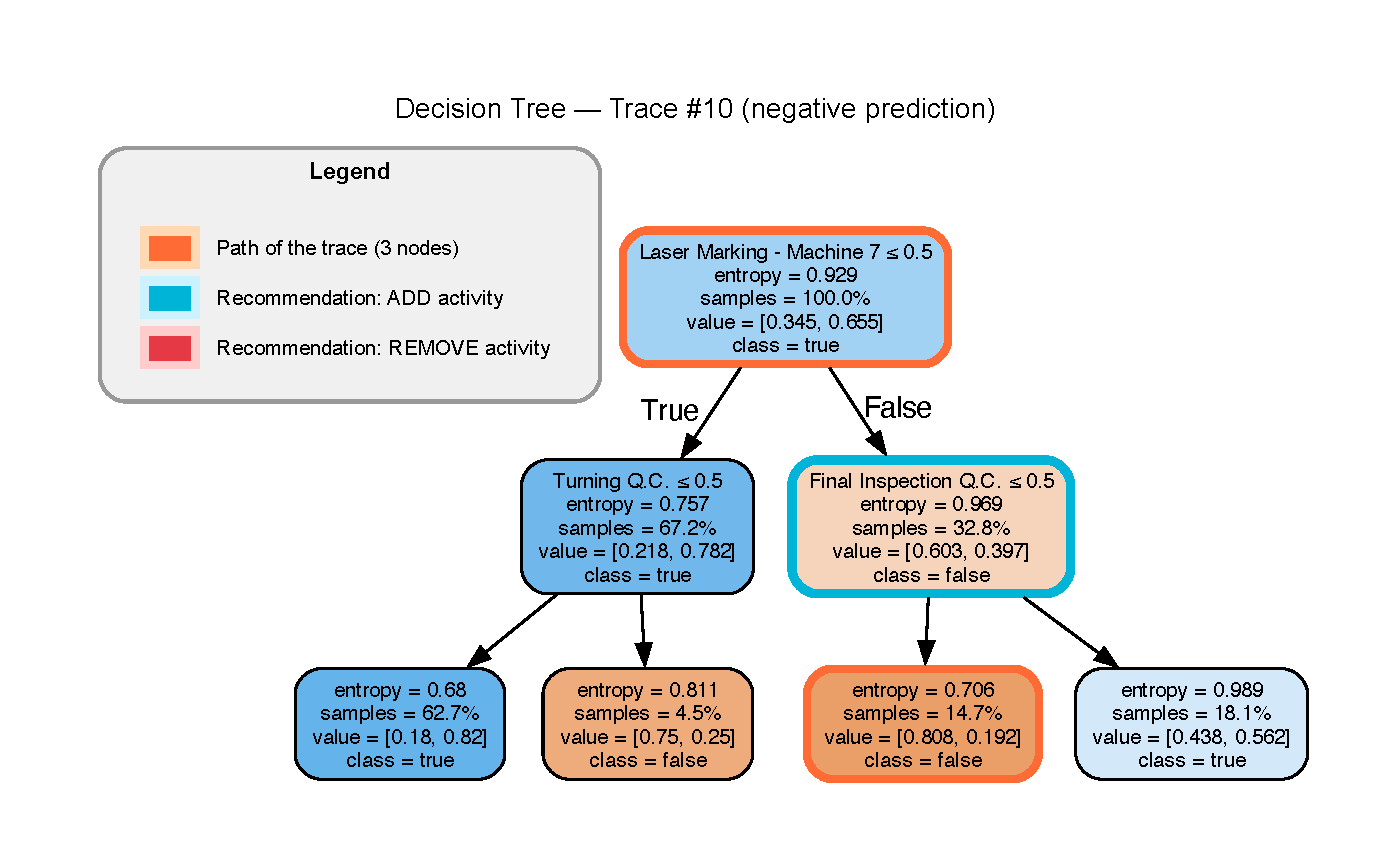
\includegraphics[width=0.95\textwidth]{annotated_tree.pdf}
    \caption{Annotated decision tree for a selected negative trace.}
    \label{fig:annotated-tree}
\end{figure}

\subsection{Recommendation Evaluation}

The recommendations were evaluated against the complete (non-truncated) test traces and this produced the following confusion matrix:

\begin{center}
\begin{tabular}{cc|c|c|}
& \multicolumn{1}{c}{} & \multicolumn{2}{c}{\textbf{Ground Truth}} \\
& \multicolumn{1}{c}{} & \multicolumn{1}{c}{Negative}  & \multicolumn{1}{c}{Positive} \\\cline{3-4}
\multirow{2}{*}{\textbf{Recommendation}} & Followed     & 1 (FP) & 1 (TP) \\\cline{3-4}
                                          & Not Followed & 4 (TN) & 1 (FN) \\\cline{3-4}
\end{tabular}
\end{center}

\vspace{0.5cm}

\begin{center}
\begin{tabular}{lr}
\toprule
\textbf{Metric} & \textbf{Value} \\
\midrule
Accuracy$_{\text{rec}}$  & 0.714 \\
Precision$_{\text{rec}}$ & 0.500 \\
Recall$_{\text{rec}}$    & 0.500 \\
F$_{\text{rec}}$         & 0.500 \\
\bottomrule
\end{tabular}
\end{center}

\noindent
The recommendation accuracy is 71.4\%, meaning that 5 out of 7 traces were classified correctly. Precision and recall are both 0.500, which is likely due to the small number of traces used in the evaluation. Specifically:

\begin{itemize}
    \item \textbf{TP = 1}: One trace followed the recommendation (the recommended activity was present in the complete trace) and indeed had a positive ground-truth outcome.
    \item \textbf{TN = 4}: Four traces did not follow the recommendation (the recommended activity was absent in the complete trace) and their ground-truth outcome was negative. These represent cases where the slow traces remained slow, consistent with not following the advice.
    \item \textbf{FP = 1}: One trace followed the recommendation but the ground-truth outcome was still negative. This indicates the recommendation was not sufficient to change the outcome.
    \item \textbf{FN = 1}: One trace did not follow the recommendation but still achieved a positive outcome, suggesting other (unmodeled) factors contributed to the positive result.
\end{itemize}

\noindent
The relatively modest $F_{\text{rec}}$ of 0.500 should be interpreted considering the very small evaluation sample (only 7 traces with negative predictions). With larger datasets, the metrics would likely stabilize and provide more reliable estimates.

\begin{figure}[H]
    \centering
    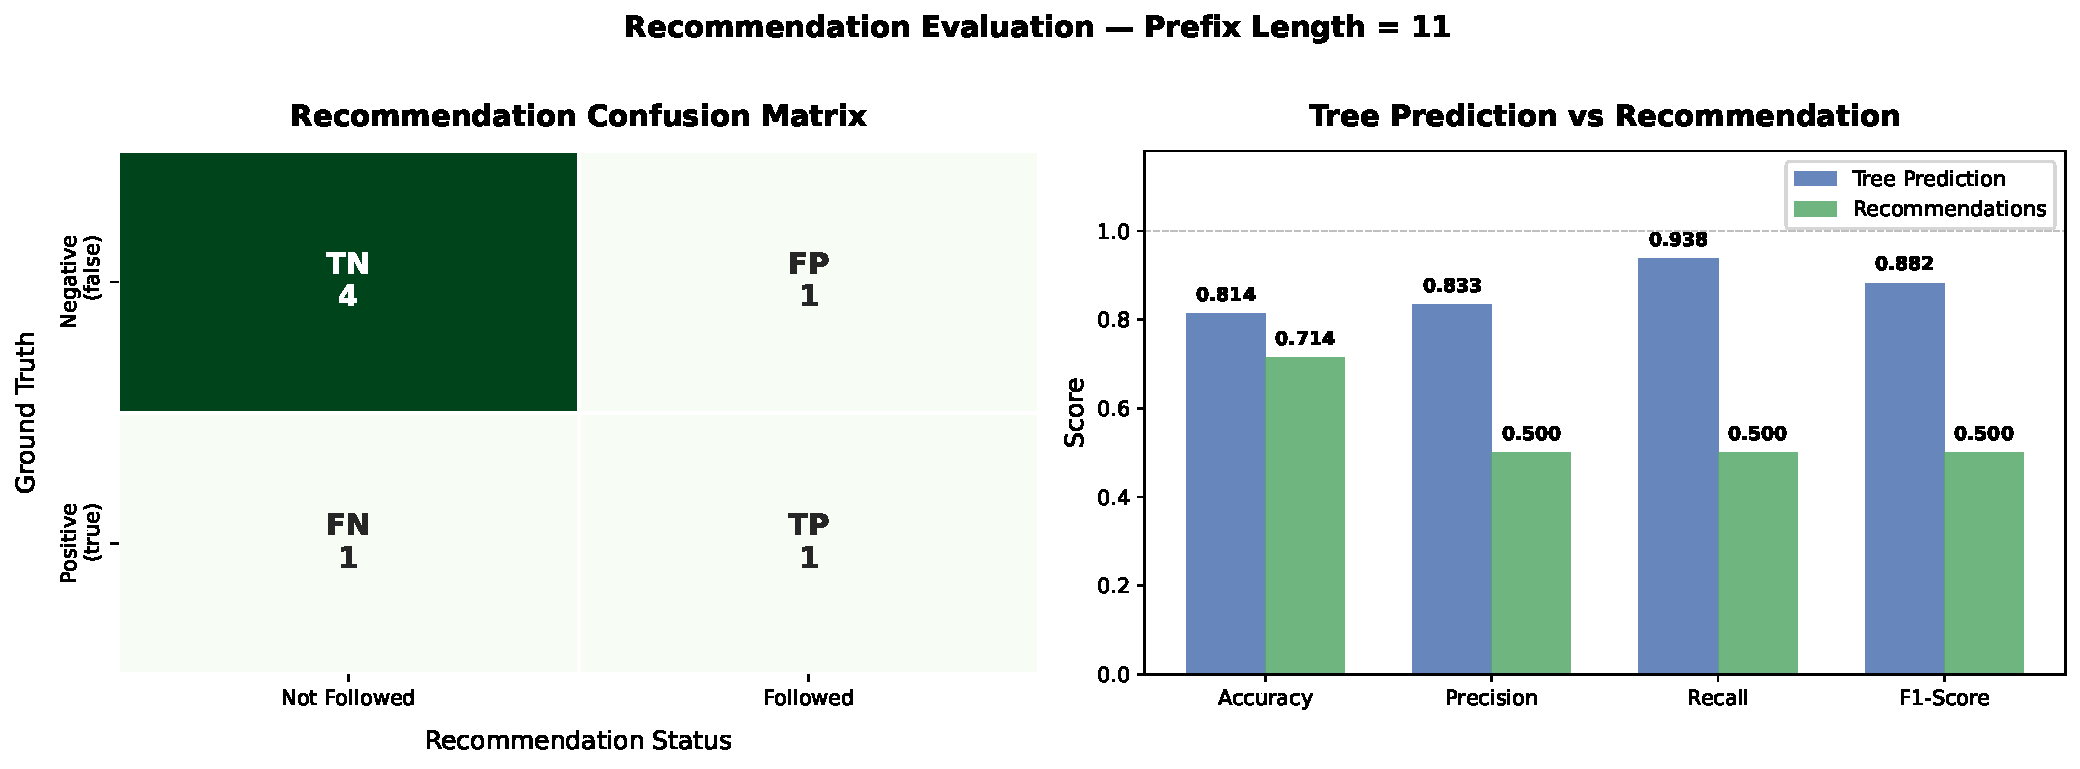
\includegraphics[width=\textwidth]{rec_evaluation.pdf}
    \caption{Recommendation evaluation results (prefix length~=~11). \textbf{Left}: Confusion matrix for the recommendation system, where the axes represent the recommendation status (followed/not followed) and the ground-truth outcome. \textbf{Right}: Side-by-side comparison of tree prediction metrics (blue) and recommendation evaluation metrics (green). The gap between the two sets of metrics reflects the additional difficulty of not only predicting the outcome correctly, but also generating recommendations that are actually followed and effective.}
    \label{fig:rec-evaluation}
\end{figure}

\subsection{Prefix Length Comparison}

To assess the impact of prefix length on both prediction and recommendation quality, the entire pipeline was executed independently for every prefix length from 1 to 12. Table~\ref{tab:prefix-comparison} reports the F1-score for both the decision tree classifier and the recommendation system, together with the number of negatively predicted traces (which determines how many traces are eligible for recommendation evaluation).

Table~\ref{tab:prefix-5-vs-11} provides a direct side-by-side comparison of the two representative prefix lengths suggested by the assignment (5 and 11), reporting all four metrics for both the decision tree classifier and the recommendation system.

\begin{table}[H]
\centering
\caption{Direct comparison of prefix lengths 5 and 11. All metrics are reported for both the decision tree prediction and the recommendation evaluation.}
\label{tab:prefix-5-vs-11}
\begin{tabular}{l rr rr}
\toprule
& \multicolumn{2}{c}{\textbf{Decision Tree}} & \multicolumn{2}{c}{\textbf{Recommendations}} \\
\cmidrule(lr){2-3} \cmidrule(lr){4-5}
\textbf{Metric} & \textbf{Prefix 5} & \textbf{Prefix 11} & \textbf{Prefix 5} & \textbf{Prefix 11} \\
\midrule
Accuracy  & 0.744 & 0.814 & 0.000 & 0.714 \\
Precision & 0.744 & 0.833 & 0.000 & 0.500 \\
Recall    & 1.000 & 0.938 & 0.000 & 0.500 \\
F1-Score  & 0.853 & 0.882 & 0.000 & 0.500 \\
\midrule
Neg.\ Predictions & 0 & 7 & --- & --- \\
\bottomrule
\end{tabular}
\end{table}

\noindent
The confusion matrices for the two prefix lengths are shown in Table~\ref{tab:cm-5-vs-11}.

\begin{table}[H]
\centering
\caption{Confusion matrices for the decision tree classifier at prefix lengths 5 and 11.}
\label{tab:cm-5-vs-11}
\begin{minipage}[t]{0.45\textwidth}
\centering
\textbf{Prefix length = 5}

\medskip
\begin{tabular}{cc|c|c|}
& \multicolumn{1}{c}{} & \multicolumn{2}{c}{\textbf{Predicted}} \\
& \multicolumn{1}{c}{} & \multicolumn{1}{c}{Neg.}  & \multicolumn{1}{c}{Pos.} \\\cline{3-4}
\multirow{2}{*}{\textbf{Actual}} & Neg. & 0 & 11 \\\cline{3-4}
                        & Pos. & 0 & 32 \\\cline{3-4}
\end{tabular}
\end{minipage}
\hfill
\begin{minipage}[t]{0.45\textwidth}
\centering
\textbf{Prefix length = 11}

\medskip
\begin{tabular}{cc|c|c|}
& \multicolumn{1}{c}{} & \multicolumn{2}{c}{\textbf{Predicted}} \\
& \multicolumn{1}{c}{} & \multicolumn{1}{c}{Neg.}  & \multicolumn{1}{c}{Pos.} \\\cline{3-4}
\multirow{2}{*}{\textbf{Actual}} & Neg. & 5 & 6 \\\cline{3-4}
                        & Pos. & 2 & 30 \\\cline{3-4}
\end{tabular}
\end{minipage}
\end{table}

\noindent
At prefix length 5, the tree predicts \textit{all} 43 traces as positive (zero negative predictions), correctly identifying all 32 fast traces (recall~=~1.0) but misclassifying all 11 slow traces as fast. With only 5 events observed, the activities in the prefix are not yet informative enough for the tree to distinguish slow from fast traces, so it defaults to predicting the majority class (positive). As a consequence, no recommendations can be extracted or evaluated, resulting in zero for all recommendation metrics.

\medskip
\noindent
At prefix length 11, the tree achieves a more balanced confusion matrix: it correctly identifies 5 out of 11 negative traces (TN~=~5) while maintaining high recall on positives (30/32). The 7 negative predictions enable the recommendation system to operate, achieving $F_{\text{rec}}$~=~0.500. This comparison shows that short prefixes do not provide enough information to identify at-risk cases, while longer prefixes allow both better classification and useful recommendations.

\medskip
\noindent
The full results across all prefix lengths 1--12 are reported in Table~\ref{tab:prefix-comparison}.

\begin{table}[H]
\centering
\caption{Decision tree and recommendation F1-scores across prefix lengths 1--12. ``Neg.~Preds'' indicates the number of test traces predicted as negative, i.e., the traces for which recommendations are generated and evaluated.}
\label{tab:prefix-comparison}
\begin{tabular}{crrrr}
\toprule
\textbf{Prefix} & \textbf{Tree Acc.} & \textbf{Tree F1} & \textbf{Rec.\ F1} & \textbf{Neg.\ Preds} \\
\midrule
1  & 0.744 & 0.853 & 0.000 & 0 \\
2  & 0.744 & 0.849 & 0.000 & 2 \\
3  & 0.744 & 0.853 & 0.000 & 0 \\
4  & 0.744 & 0.853 & 0.000 & 0 \\
5  & 0.744 & 0.853 & 0.000 & 0 \\
6  & 0.721 & 0.838 & 0.000 & 1 \\
7  & 0.744 & 0.853 & 0.000 & 0 \\
8  & 0.744 & 0.853 & 0.000 & 0 \\
9  & 0.744 & 0.825 & 0.250 & 12 \\
10 & 0.744 & 0.841 & 0.000 & 6 \\
11 & 0.814 & 0.882 & 0.500 & 7 \\
12 & 0.767 & 0.839 & 0.000 & 13 \\
\bottomrule
\end{tabular}
\end{table}

\subsubsection{Decision Tree F1 Trend}

The left panel of Figure~\ref{fig:prefix-f1} shows that the decision tree F1-score is fairly stable across prefix lengths, around 0.85. For short prefixes (1--8), the tree tends to predict the majority class (positive), achieving high F1 primarily through high recall but low discriminative power (0 or very few negative predictions). The peak is reached at \textbf{prefix length 11} (F1 = 0.882), where the tree achieves the best balance between precision (0.833) and recall (0.938). At prefix length 12, the F1 decreases slightly to 0.839, suggesting that additional events may introduce noise or reduce generalization.

\subsubsection{Recommendation F1 Trend and Negative Predictions}

The center panel of Figure~\ref{fig:prefix-f1} shows a clear pattern: the recommendation F1 is \textbf{zero for most prefix lengths} (1--8), with non-trivial values appearing only from prefix length 9 onward. The right panel explains why: it shows the number of negative predictions at each prefix length. For short prefixes (1--8), the tree predicts almost all traces as positive, producing 0 or very few negative predictions and therefore leaving no traces for which to generate and evaluate recommendations.

\medskip
\noindent
The recommendation system achieves its best performance at \textbf{prefix length 11} ($F_{\text{rec}}$ = 0.500), coinciding with the prefix length where the decision tree also achieves its highest F1. At prefix length 9, a moderate $F_{\text{rec}}$ of 0.250 emerges alongside the first substantial wave of negative predictions (12 traces).

\medskip
\noindent
Prefix lengths 10 and 12, however, show a different pattern: despite generating 6 and 13 negative predictions respectively, their recommendation F-score is 0.000. A recommendation is evaluated as a true positive only if the recommended activities actually appear in the complete trace and the ground truth is positive. A score of 0.000 therefore indicates that, for those prefix lengths, none of the negatively-predicted traces satisfied both conditions simultaneously—either the recommended activities did not appear in the remaining events of the trace, or the trace remained slow. This suggests that the quality of recommendations depends not only on the number of negative predictions, but also on whether the specific tree structure and observable features at a given prefix length produce recommendations aligned with the actual process behaviour.

\subsubsection{Key Insights}

The prefix length analysis shows the following:

\begin{itemize}
    \item \textbf{Prediction stability}: The decision tree F1-score is relatively insensitive to prefix length, remaining in the 0.82--0.88 range. 
    \item \textbf{Recommendation threshold}: Meaningful recommendations only emerge from prefix length 9 onward, when the tree begins to make a non-trivial number of negative predictions. Without enough negative predictions, there are simply no traces to recommend on.
    \item \textbf{Optimal prefix length}: Prefix length 11 is the sweet spot for this dataset, maximizing both the tree F1-score (0.882) and the recommendation F1-score (0.500).
    \item \textbf{Non-monotonic behavior}: The recommendation F1 does not increase monotonically with prefix length. Having more negative predictions (prefix 12: 13 negatives) does not guarantee better recommendation quality, suggesting that the specific tree structure and the activities observable at each prefix length play a critical role.
    \item \textbf{Negative prediction concentration}: As visible in the right panel of Figure~\ref{fig:prefix-f1}, negative predictions are heavily concentrated at prefix lengths 9--12, with a sharp jump from 0--2 (prefixes 1--8) to 6--13 (prefixes 9--12). This transition marks the point where the process has revealed enough activities for the tree to start distinguishing slow traces from fast ones.
\end{itemize}

\begin{figure}[H]
    \centering
    
\includegraphics[width=\textwidth]{prefix_f1_comparison.pdf}
    \caption{Prefix length analysis (1--12). \textbf{Left}: Decision tree F1---relatively stable around 0.85, peaking at prefix length 11 (0.882). \textbf{Center}: Recommendation system F1---zero for most short prefixes, with the best performance at prefix length 11 ($F_{\text{rec}}$ = 0.500). \textbf{Right}: Number of negative predictions per prefix length---the bar chart explains the recommendation trend: only when the tree produces a meaningful number of negative predictions (prefix $\geq$ 9) can the recommendation system be evaluated and potentially succeed.}
    \label{fig:prefix-f1}
\end{figure}


\section{Conclusion}

This project presented a complete recommendation system for predictive process monitoring, applying decision tree classifiers to a real-world production event log. The pipeline includes data preprocessing (prefix extraction with padding, boolean encoding), hyperparameter optimization via GridSearchCV, outcome prediction, recommendation extraction from the tree's internal structure, and a dedicated evaluation methodology.

\medskip
\noindent
The results show that even a shallow decision tree can achieve strong predictive performance on this dataset, while the recommendation component generates interpretable suggestions based on the tree's structure. The qualitative analysis confirms that the recommendations are consistent with the learned decision boundaries: the system correctly identifies which activities are missing from a trace's prefix and suggests adding them to move the process towards a positive outcome.

\medskip
\noindent
The prefix length comparison (1--12) revealed an important trade-off: while prediction quality remains stable across prefix lengths, the recommendation system only becomes effective when the prefix is long enough for the tree to distinguish between positive and negative traces. At the same time, very long prefixes do not guarantee better recommendations, since the remaining portion of the trace may no longer allow the recommended activities to be incorporated. This interplay between prediction and recommendation quality is a key finding of the analysis.

\medskip
\noindent
From a practical standpoint, the results suggest that the quality control steps identified by the tree are critical activities in the production process: their presence is strongly associated with faster cycle times. This insight could be used by process managers to prioritize such steps in ongoing production instances.

\subsection{Limitations and Future Works}
A limitation of this work is the relatively small test set, which limits the reliability of the recommendation evaluation metrics.

\medskip
\noindent
Moreover, it is important to note that the recommendation metric $F_{\text{rec}}$ is inherently \textbf{retrospective}: it verifies \textit{a~posteriori} whether the recommended activities happened to occur in the complete trace and whether the outcome was positive. This does not establish a \textbf{causal} relationship between performing the recommended activities and achieving a positive outcome. In other words, the metric cannot prove that the recommended activities \textit{caused} the positive result---only that they co-occurred with it. A trace may have reached a positive outcome due to factors not captured by the boolean encoding (e.g., temporal ordering, resource allocation, or external conditions). Conversely, a recommendation classified as a false positive does not necessarily mean the suggestion was wrong in general; it may simply indicate that the recommended activities alone were not sufficient under the specific circumstances of that trace. Despite this limitation, $F_{\text{rec}}$ remains a useful proxy for recommendation quality, as it measures the alignment between the system's suggestions and the actual process behavior.

\medskip
\noindent
Future work could explore larger event logs, more sophisticated models (e.g., random forests, gradient boosting), and multi-step recommendation strategies that account for the temporal ordering of activities.


\end{document}
